% ============================================================================
% CORE RESULTS — the full attention battery on the cued change-detection
% environment (vda1/vda4), affine_ew is THE model. Ledger E1, E2, E4, E5.
% The lead result of the paper and its longest section.
%   6.1 psychometrics & RT: checkpoint-specific cueing across tasks
%   6.2 attention deployment: orient-then-release, dilution, validity-blind map
%   6.3 signal detection: criterion shift AND sensitivity, both realized
%   6.4 decision uncertainty: misdirection -> confident miss
%   6.5 temporal decoding: value latched, validity cue-locked and weak post-cue,
%       change built online; the event-time position code
%   6.6 attentional microstimulation: inject priority -> false detection, gated
% Every number in this section is measured on the trained affine_ew d128
% vda1/vda4 model. NO architecture comparison; this is "the model."
% ============================================================================
\section{The model reproduces the core signatures of spatial attention in a
         cued change-detection task}
\label{sec:detection}

The lead result of this paper is that a single recurrent vision transformer with
spatial working memory, trained with reinforcement plus temporal JEPA self-supervision
(loss weight $0.5$) to report an orientation change
among cued Gabor stimuli, reproduces the behavioral, psychophysical, and
signal-detection signatures of primate spatial attention, and does so through
internal mechanisms that can be read out and causally manipulated. We subject the
canonical affine-feedback checkpoints to an exhaustive battery on the cued
change-detection environment at two set sizes --- one monitored stimulus
(\texttt{vda1}) and four (\texttt{vda4}) --- and organize the battery as six analyses: psychometrics and
reaction time (Section~\ref{sec:det-psych}); attention deployment
(Section~\ref{sec:det-attn}); signal-detection read-out
(Section~\ref{sec:det-sdt}); decision uncertainty
(Section~\ref{sec:det-uncertainty}); temporal decoding from working memory
(Section~\ref{sec:det-decoding}); and attentional microstimulation
(Section~\ref{sec:det-microstim}). Each analysis states the finding, the measured
number that supports it, and the human or primate result it reproduces.

The model is competent on the task at the checkpoint analyzed throughout: it is
correct on approximately $0.83$ of natural trials, and its detection is a graded
function of change magnitude in every cue condition (Section~\ref{sec:det-psych}).
The detailed causal and decoding results use the canonical \texttt{vda4}
$d_{\mathrm{mem}}=128$ checkpoint; the set-size comparison adds a separately trained
\texttt{vda1} checkpoint with the same affine-feedback mechanism. Where an analysis
applies an attention clamp, we say so explicitly and
give the clamp range; unclamped ("natural") numbers are the model's spontaneous
behavior.

% ---------------------------------------------------------------------
\subsection{Psychometrics and reaction time across task checkpoints}
\label{sec:det-psych}

The first analysis establishes that the model is a graded detector and that a
spatial-cueing benefit is present in the canonical four-stimulus checkpoint. A
separately trained single-stimulus checkpoint lacks a comparable cued-versus-uncued
contrast; this two-checkpoint observation motivates, but does not establish, a
noise-limited set-size law.

\paragraph{Detection is a graded psychometric function, and reaction time falls
with change magnitude.}
In every cue condition the probability of reporting a change is a monotone
psychometric function of the orientation-change magnitude $|\Delta\theta|$, and the
model responds faster (presses earlier relative to the change frame) for larger
$|\Delta\theta|$. These are the two elementary behavioral signatures of a graded
evidence-accumulating detector: a smooth magnitude--detection curve and a
magnitude--latency trade-off. They hold at both set sizes and are the substrate on
which the cueing manipulations act.

\paragraph{The cueing contrast differs across separately trained tasks.}
The spatial-cueing benefit --- the leftward shift of the psychometric function (a
lower detection threshold) for cued relative to uncued changes --- is visible in
the canonical \texttt{vda4} evaluation. VDA1 has no uncued active item and therefore
does not define the same spatial contrast. The four-checkpoint battery in
Section~\ref{sec:vda-battery} reports a different quantity: low- minus high-validity
\emph{cued-threshold} change. Its VDA9 value is $2.207^\circ$ and must not be read as
a cued-versus-uncued benefit. The current cross-checkpoint observations are
compatible with a role for competition and spatial uncertainty
\cite{carrasco2011_visual_attention_25y}, but do not isolate set size.

\paragraph{A genuine spatial benefit, at threshold magnitudes.}
The benefit is present at diagnostic (threshold) change magnitudes and is spatial in
origin: at full ring completeness and a threshold step of $|\Delta\theta| =
16^\circ$, the model detects the change on $0.43$ of validly cued trials but only
$0.21$ of invalidly cued trials --- a doubling of detection for a change at the
monitored location. This is the model-level counterpart of the classic Posner
cueing benefit: processing is enhanced at the location a spatial cue directs
attention toward \cite{posner1980_orienting}.

\paragraph{The benefit is flat across cue validity.}
Critically, the size of the cueing benefit does not scale with how predictive the
cue is. Sweeping the displayed cue validity (the ring-completeness proportion $p \in
\{0.25, 0.5, 0.75, 1.0\}$, i.e.\ how often the cue correctly marks the changing
location), the valid$-$invalid detection gap at threshold magnitudes
($12$--$20^\circ$) is essentially constant across proportions: $0.21$, $0.23$,
$0.19$, $0.25$ at $p = 0.25, 0.5, 0.75, 1.0$ respectively. The model gains from
being told \emph{where} to look, but not from being told \emph{how reliable} that
instruction is. This validity-blindness is a behavioral fact whose internal
mechanism the decoding analysis constrains directly: the validity signal is strongest
at the cue and only weakly recoverable afterward (Section~\ref{sec:det-decoding}). It
also connects the model to the normative prediction that a high-validity design
carries a negligible value-directed-attention benefit; the model's flat cueing
benefit across proportion is the empirical face of that regime.

\begin{figure}[t]
  \centering
  % FIGURE: per-cue-condition psychometric curves P(detect) vs |Delta theta|,
  % plus RT-vs-Delta, plus valid-invalid gap vs proportion. Render from the
  % vda_sweep psychometrics npz (vda4 affine_ew) -> vda_fig_psych panels.
  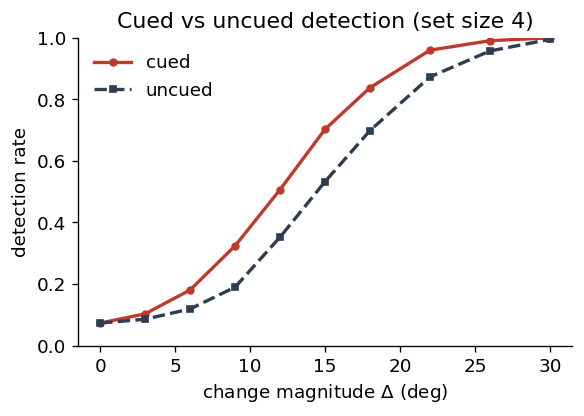
\includegraphics[width=0.95\linewidth]{figures/detection_psychometrics.png}
  \caption{Psychometrics and reaction time on the cued change-detection task
  (\texttt{vda4}, the model). \textbf{(a)} Detection probability is a graded
  monotone function of change magnitude $|\Delta\theta|$ in every cue condition;
  the cued curve is shifted left of the uncued curve (a spatial cueing benefit;
  no $2.207^\circ$ claim is made here). \textbf{(b)} Reaction time falls with
  $|\Delta\theta|$. \textbf{(c)} The valid$-$invalid detection gap at threshold
  magnitudes is flat across displayed cue validity $p$ ($0.21, 0.23, 0.19, 0.25$
  at $p = 0.25, 0.5, 0.75, 1.0$): the benefit is spatial, not validity-graded.}
  \label{fig:det-psych}
\end{figure}

% ---------------------------------------------------------------------
\subsection{Attention deployment: orient, release, re-acquire, and lock ---
            diluted by load, blind to validity, and not shaped by value}
\label{sec:det-attn}

The second analysis reads the model's attention map directly. Because the model
attends over the stimulus patches with a softmax, the per-patch attention weight is
a priority map: the weight on the cued patch, $\alpha_1$ (uniform baseline $0.25$
for four patches), measures how much the model is monitoring the cued location at
each frame. Averaging the attention map over trials per condition ($96$ trials per
condition; weights reported raw, without renormalization) gives a frame-by-frame
time-course of where the model is looking.

\paragraph{A legible attentional schedule: transient orient, release, re-acquire,
bottom-up lock.}
The model deploys attention on a four-phase schedule. (i) \emph{Orient:} at the cue
frame ($t = 1$) attention to the cued patch rises to $\alpha_1 = 0.73$, far above
the uniform baseline of $0.25$ --- the model orients to the location the cue marks.
(ii) \emph{Release:} during the following blank ($t = 2$) attention falls back to
chance ($\alpha_1 = 0.22$) --- the model does not hold a tight spatial focus through
the empty delay. (iii) \emph{Re-acquire:} as the Gabor array appears the model
re-acquires the cued location, with $\alpha_1$ rising from $0.44$ to $0.80$ across
$t = 3, 4$. (iv) \emph{Lock:} when a change occurs, attention approaches the top of its sampled
range on the changed patch. This orient--release--re-acquire schedule is a model-level rendering
of transient, then later cue-directed, covert spatial orienting. Because no
cue-location decoder was fitted across the blank, re-acquisition is compatible
with an intervening memory trace but does not demonstrate decoded cue-location maintenance.

\paragraph{The change-lock is bottom-up: it captures valid and invalid changes
alike.}
When a change occurs, attention locks onto the changed patch on the change frame
($t = 5$) regardless of whether that patch was cued: attention to the changed patch
is $1.00$ for a validly cued change and $0.92$ for an invalidly cued change, decaying
by the following frame ($0.71$ valid, $0.54$ invalid at $t = 6$). A large orientation
step pulls attention wherever it occurs --- a bottom-up salience grab that operates
in parallel with the top-down cue-driven orienting. This bottom-up capture is why
the behavioral cueing benefit is modest rather than all-or-none: invalid changes are
still attended and therefore still frequently detected.

\paragraph{Sustained monitoring differs between the VDA1 and VDA4 checkpoints.}
The re-acquired component of attention on the cued patch is higher in the separately
trained \texttt{vda1} checkpoint than in \texttt{vda4}. This is compatible with a
resource-dilution account \cite{reynolds_heeger2009_normalization,
carrasco2011_visual_attention_25y}, but two checkpoints with different active-item
support do not establish monotonic dilution. The full battery confirms that sustained
attention is not a monotone four-point ladder (Section~\ref{sec:vda-map}).

\paragraph{The attention map is blind to cue validity.}
Exercising the validity manipulation fully --- valid and invalid changes at every
displayed proportion --- the attention map is flat across cue validity. The cue-time
focus stays at $\alpha_1 \approx 0.72$, the stimulus-phase monitoring of the cued
patch at $\approx 0.62$, and the change-time lock (valid and invalid) is unchanged
across $p \in \{0.25, \ldots, 1.0\}$. The model does not broaden its spatial
monitoring when the cue is unreliable. The predictiveness of the cue does not shape
\emph{where} attention goes --- the deployment-level counterpart of the flat
behavioral cueing benefit (Section~\ref{sec:det-psych}), and, as
Section~\ref{sec:det-decoding} shows, accompanies weak post-cue linear recoverability
of the validity signal.

\paragraph{Value is not written into the attention map.}
The cued patch's colour signals its value, but the value ordering does not appear in
the attention map. The cue-frame focus varies with cue \emph{colour} --- $\alpha_1 =
0.89$ (blue), $0.74$ (green), $0.73$ (red) --- but not monotonically with value, so
the variation is a low-level colour-appearance effect on the visual front-end rather
than a value-driven attentional gain; the change-lock is essentially value-invariant.
Value therefore does not modulate \emph{where} attention is deployed. As
Section~\ref{sec:det-decoding} shows, value is nonetheless retained in working
memory and reaches the decision --- a deployment-versus-use dissociation that
distinguishes value (retained and usable, but not in the map) from validity
(perceived, then discarded). The interpretation of value-directed attention as a
use-stage rather than a deployment-stage effect is developed in
Section~\ref{sec:value}.

\begin{figure}[t]
  \centering
  % FIGURE: alpha_1 time-course (orient/release/re-acquire) + change-lock valid vs
  % invalid; plus flat-across-proportion panel; plus value/colour panel. Render
  % from vda_sweep alpha1_lines + super_vda4_affine_ew_{red,green,blue} +
  % deepdive_affine dda_timecourse / dda_prop_attn_metrics / dda_value.
  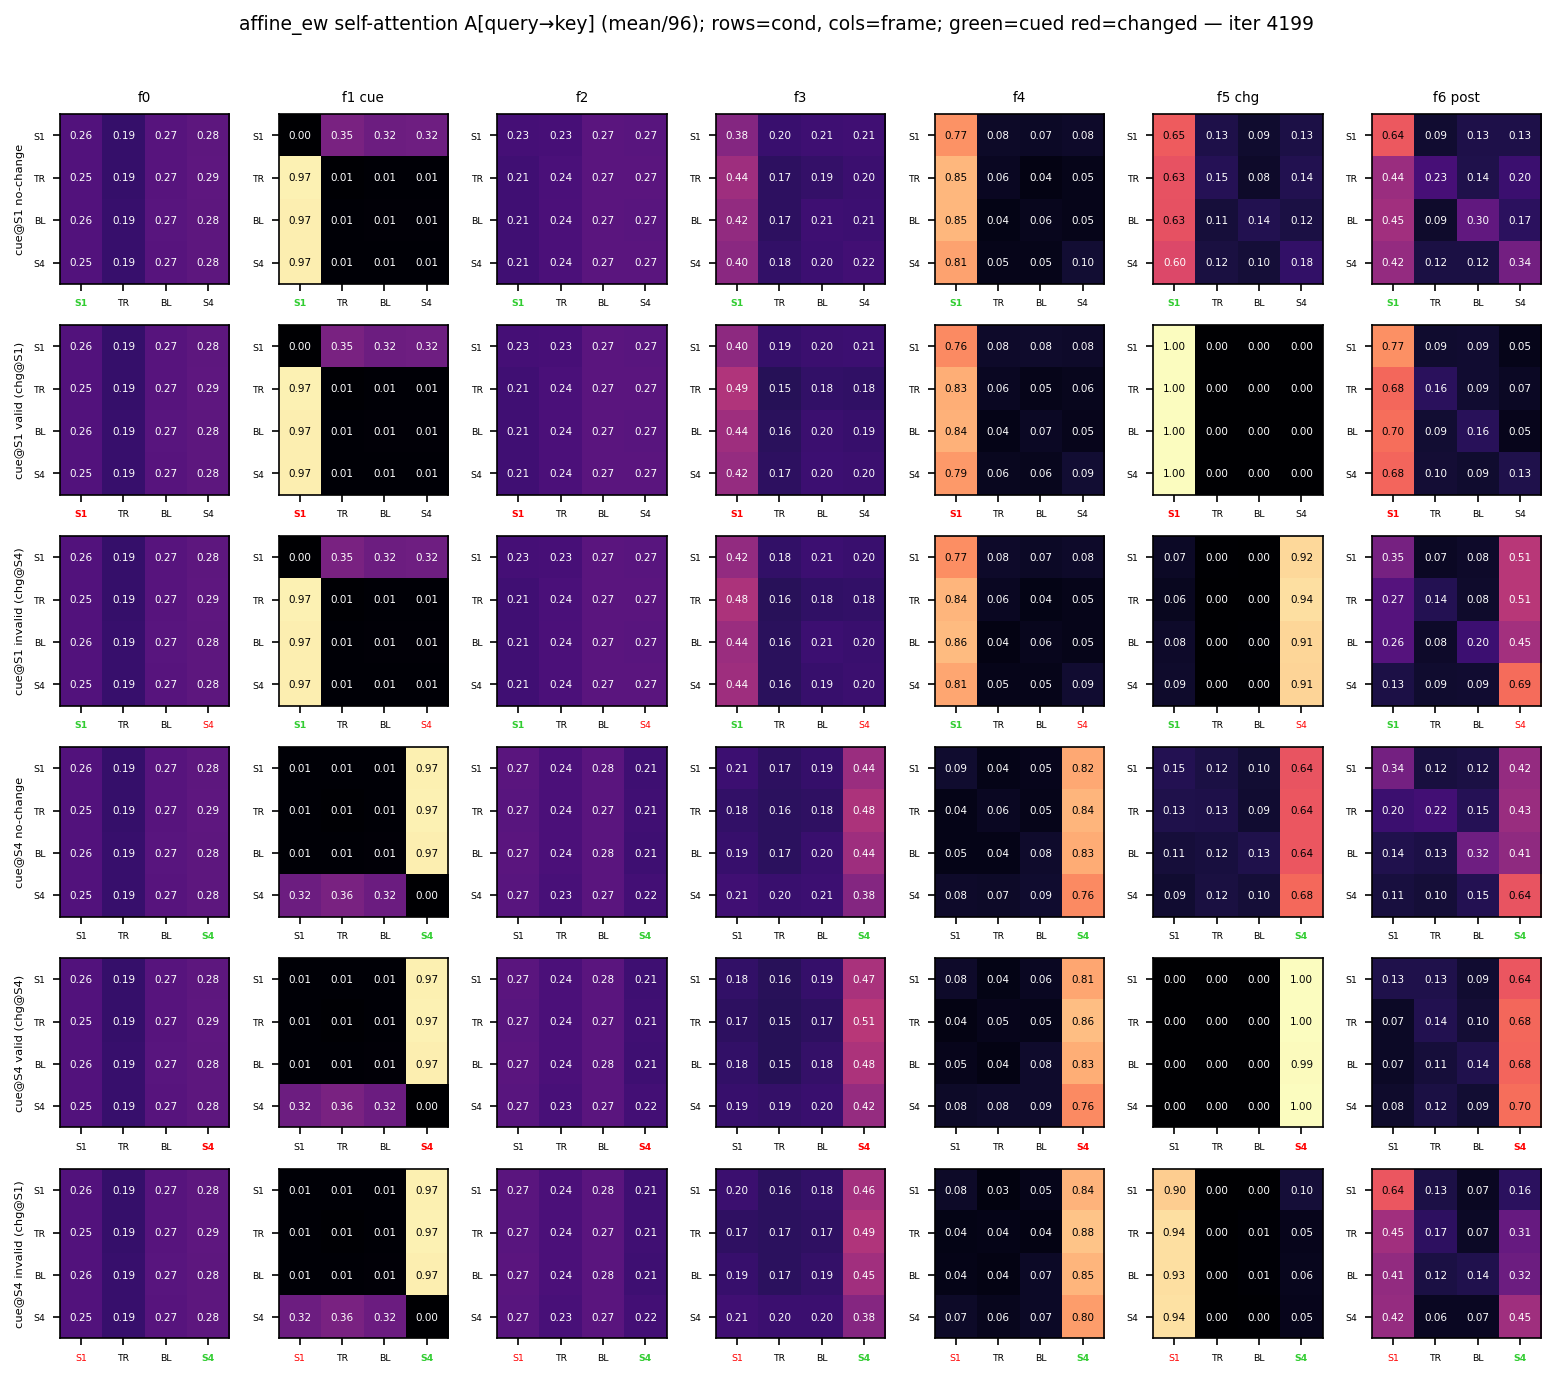
\includegraphics[width=0.95\linewidth]{figures/detection_attention.png}
  \caption{Attention deployment (the model). \textbf{(a)} The $\alpha_1$
  time-course: orient at the cue ($0.73$ at $t=1$), release at the blank ($0.22$ at
  $t=2$), re-acquire over the Gabor frames ($0.44 \to 0.80$), lock at the change.
  \textbf{(b)} The change-lock is bottom-up: attention to the changed patch at
  $t=5$ is $1.00$ (valid) and $0.92$ (invalid). \textbf{(c)} The map is flat across
  displayed cue validity. \textbf{(d)} Sustained monitoring dilutes from
  \texttt{vda1} to \texttt{vda4}. Uniform baseline $\alpha_1 = 0.25$ throughout.}
  \label{fig:det-attn}
\end{figure}

\begin{figure}[t]
  \centering
  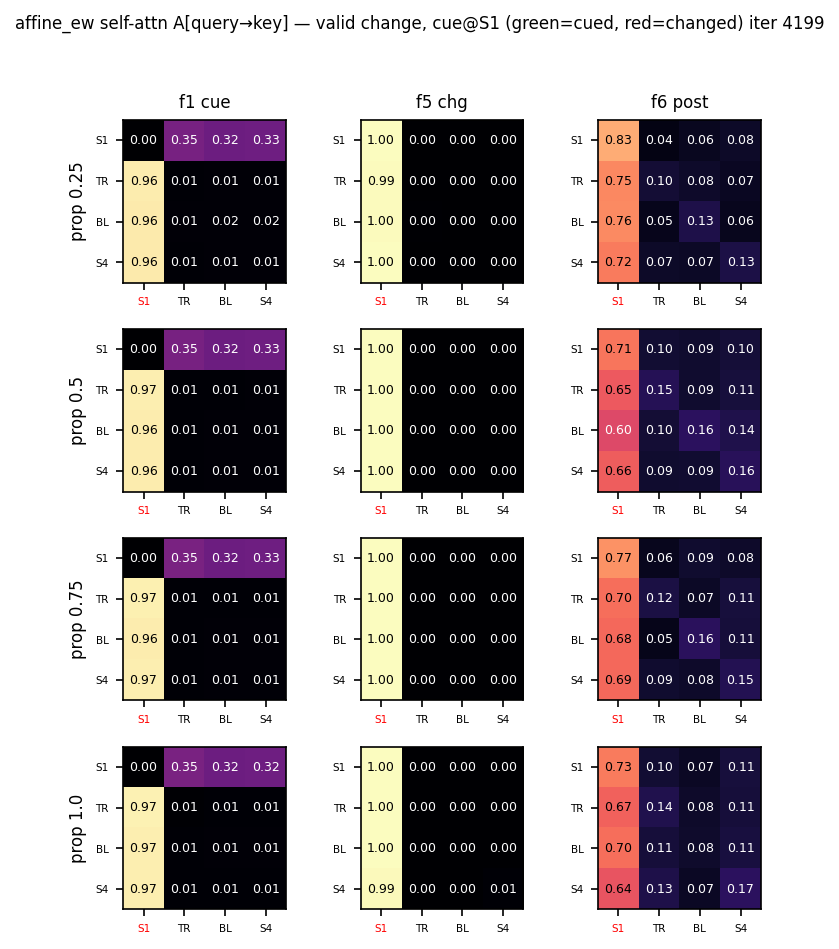
\includegraphics[width=0.49\linewidth]{figures/fig_attn_maps_valid.png}\hfill
  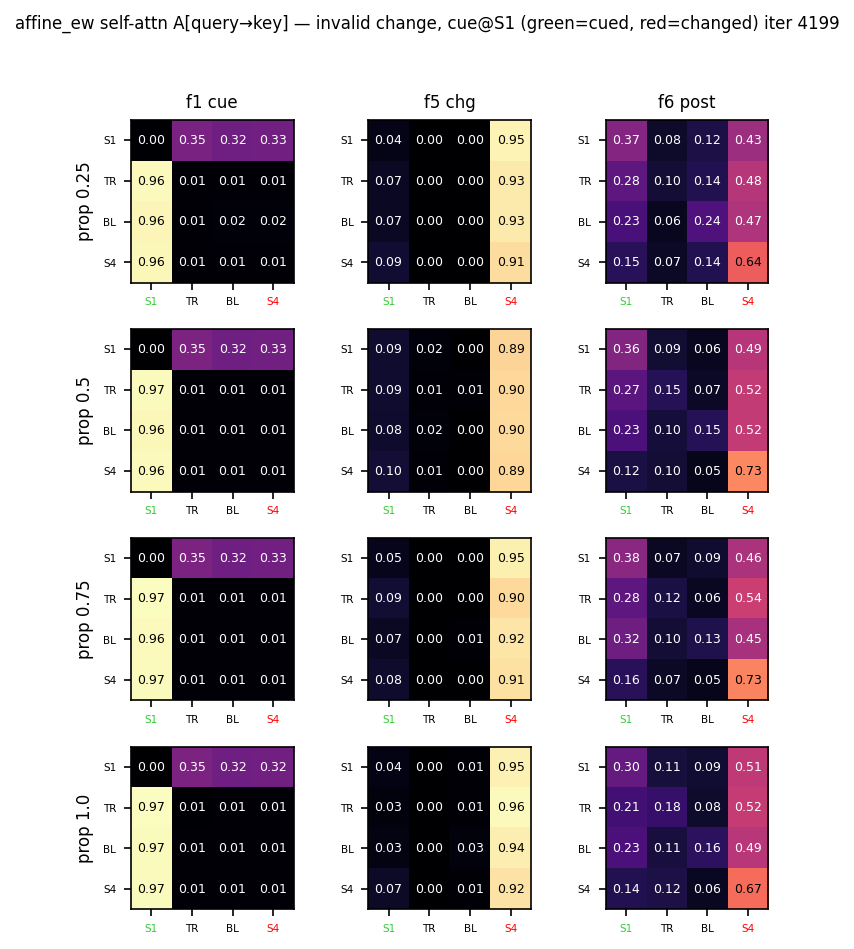
\includegraphics[width=0.49\linewidth]{figures/fig_attn_maps_invalid.png}\\[4pt]
  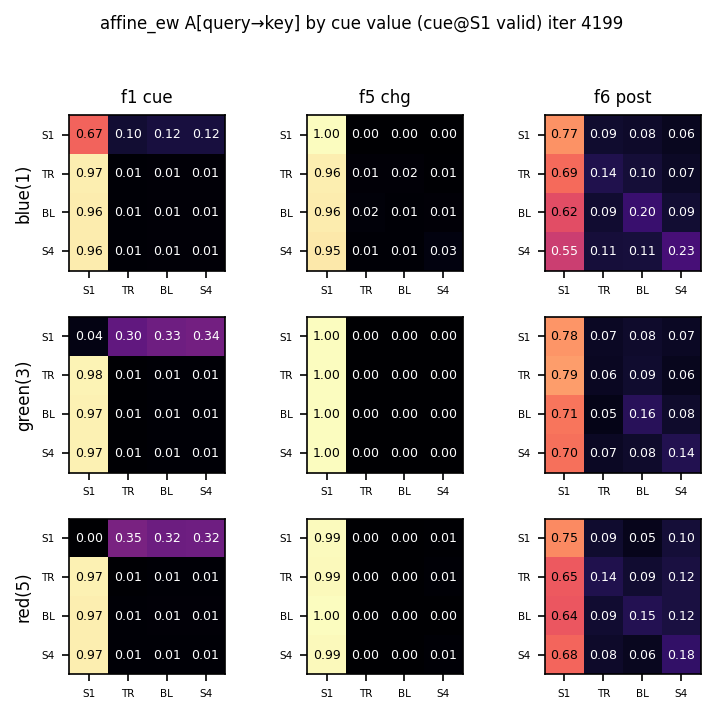
\includegraphics[width=0.49\linewidth]{figures/fig_attn_value_maps.png}\hfill
  
\includegraphics[width=0.49\linewidth]{figures/fig_attn_timecourse.png}
  \caption{\textbf{Attention maps of the model, conditioned on cue validity and value.}
  \emph{Top:} the per-patch attention map across the trial on validly cued (left) and
  invalidly cued (right) trials, resolved by displayed cue proportion --- attention
  orients to the cue and then locks onto the changed patch. \emph{Bottom left:} the
  attention maps split by cue colour (value) are essentially indistinguishable ---
  value is \emph{not} written into the priority map. \emph{Bottom right:} the
  $\alpha_c$ time-course underlying the maps (orient; release at the blank; re-acquire;
  lock). All panels are the model (affine feedback) on \texttt{vda4}.}
  \label{fig:det-attn-maps}
\end{figure}

% ---------------------------------------------------------------------
\subsection{Signal-detection read-out: attention lowers the criterion \emph{and}
            raises sensitivity}
\label{sec:det-sdt}

The third analysis is the paper's central signal-detection result. It asks what
attention does to detection in the terms the primate literature uses --- the
decision criterion $c$ and the perceptual sensitivity $d'$ --- by sweeping the
attention bias on the cued patch and reading out both quantities. We sweep a nominal clamp setting on the cued key from suppression to enhancement;
the analysis maps that setting to an additive pre-softmax logit bias. The nominal
setting is not a measured attention share. We then compute the hit and
false-alarm rates from which $c$ and $d'$ follow.

\paragraph{Attention lowers the decision criterion.}
Sensitivity aside, attention makes the model a more liberal detector. Across the sampled clamp settings in the canonical \texttt{vda4} analysis, the
criterion $c$ falls monotonically from $c = 1.42$ under suppression to $c = -0.60$
under enhancement. Enhancing attention lowers the evidence threshold for reporting a
change; suppressing it raises the threshold. This is the textbook attentional
criterion shift: attention biases the observer toward detection independently of any
change in the underlying discriminability \cite{carrasco2011_visual_attention_25y}.

\paragraph{Attention is also load-bearing for sensitivity.}
Sensitivity is not merely along for the ride. Suppressing attention on the cued
patch collapses the model's discriminability --- $d'$ falls to $0.63$--$1.45$ under
suppression --- and restoring attention to its natural or enhanced level recovers it
to $d' \approx 2.0$--$2.7$. The model cannot discriminate a change it is not
attending: its perceptual sensitivity is set by where attention is deployed. This is
the sensitivity (gain) account of attention --- attention multiplies the effective
signal, raising $d'$ --- the model-level counterpart of attentional response-gain
and contrast-gain effects in visual cortex \cite{reynolds_heeger2009_normalization,
mcadams_maunsell1999_v4_tuning}, and of the sharpening of tuning and enhancement of
neuronal sensitivity under attention \cite{treue_martinez_trujillo1999_feature_attention}.

\paragraph{The model realizes both accounts in one system.}
The two effects coexist in the same clamp sweep: moving attention on the cued patch
both shifts the criterion (from $1.42$ to $-0.60$) and moves the sensitivity (from
$0.63$--$1.45$ suppressed to $\sim\!2.0$--$2.7$ restored). The long-standing debate
over whether spatial attention improves detection by shifting the decision criterion
or by improving perceptual sensitivity \cite{carrasco2011_visual_attention_25y} is,
in this model, not a dichotomy: a single manipulation of a single attentional
variable produces both a criterion shift and a sensitivity change. That both are
present and both are driven by the same attentional clamp is the central mechanistic
claim of the section --- the model instantiates the criterion account and the
sensitivity account simultaneously, and the canonical primate task that dissociates
them behaviorally is taken up in Section~\ref{sec:luomaunsell}.

\begin{figure}[t]
  \centering
  % FIGURE: c(alpha_1) and d'(alpha_1) under the graded cued-patch attention clamp,
  % vda4 affine_ew. Render from vda_sweep sdt_curves (sdt npz).
  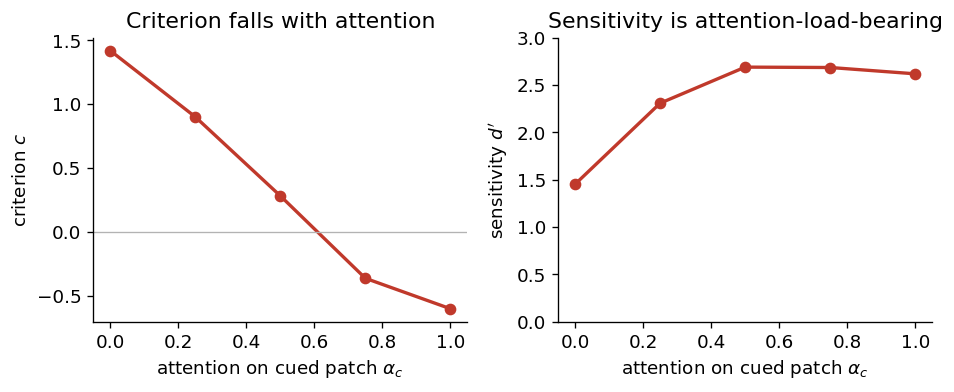
\includegraphics[width=0.8\linewidth]{figures/detection_sdt_curves.png}
  \caption{Signal-detection read-out under the graded cued-patch attention clamp
  (\texttt{vda4}, the model). \textbf{Left:} at these sampled VDA4 settings, the criterion $c$ falls monotonically
  with attention, from $1.42$ (suppress) to $-0.60$ (enhance) --- attention makes
  the detector more liberal. \textbf{Right:} sensitivity $d'$ is attention-mediated,
  collapsing to $0.63$--$1.45$ under suppression and recovering to $\sim\!2.0$--$2.7$
  under natural/enhanced attention. Both the criterion and the sensitivity account
  are realized by one manipulation.}
  \label{fig:det-sdt}
\end{figure}

% ---------------------------------------------------------------------
\subsection{Decision uncertainty: misdirected attention manufactures a confident
            miss}
\label{sec:det-uncertainty}

The fourth analysis turns to the model's internal report of its own uncertainty. The
policy's action distribution has an entropy (how undecided the model is between
\texttt{wait} and \texttt{declare-}\allowbreak\texttt{change}), and the distributional critic carries a
spread of return quantiles (how uncertain the value estimate is). We use these to ask
what happens to the model's confidence when its attention is misallocated on a trial
that in fact contains a change.

\paragraph{Misdirection produces a miss --- and, diagnostically, a confident one.}
On a real change at the uncued patch, we compare three attention conditions: attend
the change, attend nothing in particular, and misdirect attention onto the (empty)
cued patch. Misdirection produces the diagnostic failure. When attention is
misdirected, the model's probability of declaring the change falls from $0.68$ to
$0.24$ --- it misses the change because it is looking in the wrong place. But its
policy entropy \emph{falls} at the same time, from $0.053$ to $0.035$: the model
becomes \emph{more} confident precisely as it becomes wrong. It reports "no change"
with increased certainty, because misdirected attention starves the decision of the
evidence that would have made it hesitate. This is a mechanistic, model-level account
of a familiar perceptual failure --- that misallocated attention produces not just
errors but \emph{confident} errors, the signature of an inattentional miss.

\paragraph{The value system registers the problem the policy commits to.}
A finer read shows the two internal channels come apart under misdirection: even as
the policy grows more confident, the distributional critic's quantile spread
\emph{widens} --- the value system registers that something is off while the policy
commits to "no change." The confident miss is therefore a property of the action
policy specifically, not of the whole internal state: the machinery that assigns
value to the situation still carries the uncertainty that the report has discarded.
This dissociation --- a decisive but wrong policy over a value estimate that "knows"
it is unsure --- is a concrete prediction the model makes about the internal
structure of confident perceptual errors.

\begin{figure}[t]
  \centering
  % FIGURE: declare rate + policy entropy + critic quantile spread across the three
  % attention conditions (attend-change / neutral / misdirect), real change at the
  % uncued patch, vda4 affine_ew. Render from vda_sweep entropy.npz -> vda_fig_entropy.
  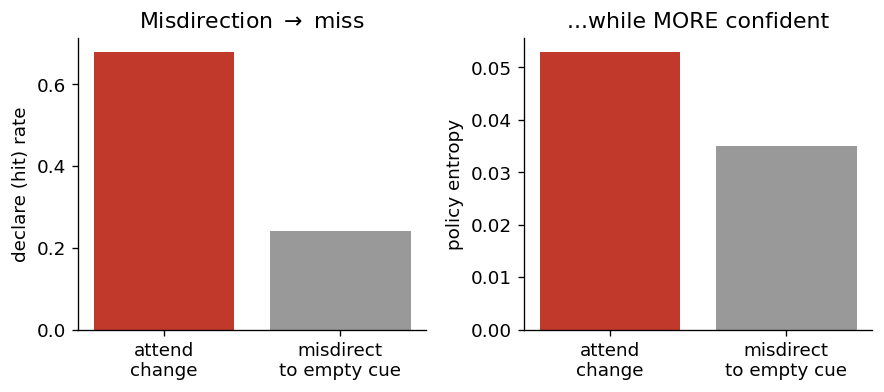
\includegraphics[width=0.9\linewidth]{figures/detection_uncertainty.png}
  \caption{Decision uncertainty under attention misdirection (real change at the
  uncued patch, the model). Misdirecting attention onto the empty cued patch drops
  the declare rate from $0.68$ to $0.24$ (a miss) while lowering policy entropy from
  $0.053$ to $0.035$ (increased confidence) --- a confident miss. The critic's
  quantile spread widens under misdirection, so the value system registers the
  problem the policy commits to.}
  \label{fig:det-uncertainty}
\end{figure}

% ---------------------------------------------------------------------
\subsection{Temporal decoding from working memory: value is latched, validity becomes
            weakly recoverable after the cue, and the change is built online}
\label{sec:det-decoding}

The fifth analysis opens the recurrent memory. Decoding the task variables from the
model's working-memory state at each frame (cross-validated logistic regression on
the flattened recurrent cell) estimates which labels are linearly recoverable at the
sampled frames. This is
the mechanistic capstone of the battery: it explains the behavioral and attentional
findings above from the internal economy of the memory, and it exposes the model's
parietal-like spatial code.

\paragraph{Value (cue colour) is latched at the cue and held.}
The cued location's value, signalled by cue colour, is decoded from the memory at
ceiling --- balanced accuracy $1.00$ --- from the cue frame ($t = 1$) through to the
change frame. Once read, value is maintained perfectly for the rest of the trial. It
is therefore available to the decision throughout, which is why value can modulate
detection (Section~\ref{sec:value}) even though it never enters the attention map
(Section~\ref{sec:det-attn}).

\paragraph{Validity is cue-locked and weakly recoverable after the cue.}
The displayed cue validity (ring proportion) is recoverable most strongly at the cue:
balanced accuracy is $0.773$ at $t=1$ and falls to $0.296$ at the blank frame
($t=2$), close to four-way chance ($0.25$). It remains near chance thereafter
(mean $t=2$--$6$: $0.309$). Thus the canonical probe supports a cue-locked validity
code followed by weak post-cue recoverability. This profile is compatible with the weak validity dependence in
the behavioral and attention-map analyses, but probe accuracy alone does not identify
the causal mechanism. The result distinguishes validity (strongest at the cue, weak
thereafter) from value (recoverable at ceiling throughout the sampled frames).

\paragraph{Change presence and location are constructed online.}
Neither the presence nor the location of the change is represented before it occurs:
both decode at chance through the pre-change frames and jump only at the change frame
($t = 5$), with change presence decodable at $0.81$ and change location at $0.50$,
rising further at $t = 6$. The memory builds the change representation as the change
happens, rather than anticipating it. That the location code is decodable and
position-specific, and becomes decodable at the sampled change frame, makes it a candidate model analogue of a
parietal priority map: a spatially organized memory of \emph{where} the behaviorally
relevant event is, active when that event is present in these sampled trials
\cite{RuffCohen2016, Srinath2021}. The timing across the three variables --- value
from the cue onward, validity briefly at the cue, change at the change frame --- shows
the memory holds what matters, when it matters, and only that.

\begin{figure}[t]
  \centering
  % FIGURE: balanced-accuracy vs timestep for value, validity, change-presence,
  % change-location, vda4 affine_ew. Render from vda_sweep decode_curves (decode
  % npz) + deepdive_affine dda_decoding.
  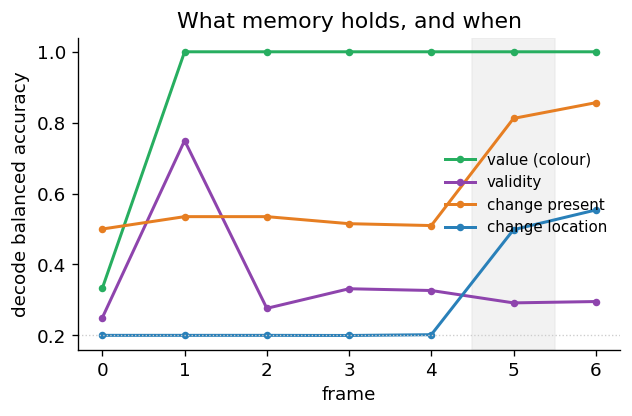
\includegraphics[width=0.9\linewidth]{figures/detection_decoding.png}
  \caption{Temporal decoding of task variables from the recurrent working-memory
  state (the model). Value (cue colour) is latched at the cue and held at balanced
  accuracy $1.00$. Validity (ring proportion) peaks at the cue ($0.773$ at $t=1$),
  falls near chance at the blank ($0.296$ at $t=2$), and remains weak thereafter
  (mean $t=2$--$6$: $0.309$). Change
  presence ($0.81$ at $t=5$) and change location ($0.50$ at $t=5$) are flat at
  chance until the change frame, then jump: the change is built online. The
  position-specific post-change code is compatible with a parietal-like event-location signal;
  no cue-location decoder was fitted across the delay.}
  \label{fig:det-decoding}
\end{figure}

% ---------------------------------------------------------------------
\subsection{Attentional microstimulation: injecting priority evokes a false
            detection, gated to the monitored location}
\label{sec:det-microstim}

The sixth analysis is a causal test. Section~\ref{sec:det-sdt} showed that removing
attention removes sensitivity and that adding attention lowers the criterion; the
converse question is whether injecting attention where the model is already
monitoring can \emph{conjure} a percept. On no-change trials we inject additional
attention (add priority to a patch's attention weight) and measure the false-detection
rate as a function of injection strength, comparing injection at the cued (monitored)
patch against injection at an uncued patch.

\paragraph{Injecting priority at the monitored location evokes false detections.}
Injecting attention onto the cued patch on no-change trials drives false detections:
the false-alarm rate rises monotonically with injection strength, from
$\approx\!0.03$ at baseline to $\approx\!0.12$ at strong injection --- roughly a
four-fold increase in reports of a change that did not occur. Surplus priority at the
monitored location is read by the downstream decision as evidence for a change. This
is the causal converse of the criterion shift of Section~\ref{sec:det-sdt}: there,
enhancing attention lowered the criterion; here, injecting attention on an empty
patch pushes the model past the criterion into a false report.

\paragraph{The evoked percept is spatially gated.}
The effect is confined to where the model is already monitoring. Injecting the same
attention at an \emph{uncued} patch does essentially nothing --- the false-alarm rate
stays flat ($\approx\!0.05$--$0.10$) across injection strength. The evoked false
detection is spatially gated to the monitored location: priority conjures a percept
only where the model is attending, not wherever it is injected. This location-gated
causal effect is the model analogue of evoking or biasing detections by
microstimulating a spatial priority map in parietal cortex or superior colliculus,
where stimulation shifts detection and choice toward the stimulated location's
receptive field \cite{RuffCohen2016}. It is also the within-task bridge to the
canonical primate paradigm of Section~\ref{sec:luomaunsell}, where the same
attention-clamp machinery reproduces the sensitivity/criterion dissociation of Luo
and Maunsell \cite{luo_maunsell2018_criterion_sensitivity}.

\begin{figure}[t]
  \centering
  % FIGURE: false-detection rate vs injected-attention strength, cued vs uncued
  % injection site, no-change trials, vda4 affine_ew. Render from vda_sweep
  % microstim_curves (microstim npz).
  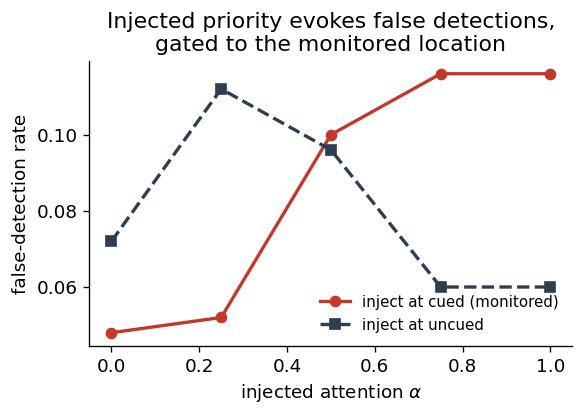
\includegraphics[width=0.8\linewidth]{figures/detection_microstim.png}
  \caption{Attentional microstimulation on no-change trials (the model). Injecting
  attention at the cued (monitored) patch drives the false-detection rate from
  $\approx\!0.03$ to $\approx\!0.12$ (a $\sim\!4\times$ increase); injecting the same
  attention at an uncued patch leaves it flat ($\approx\!0.05$--$0.10$). The evoked
  false percept is spatially gated to the location the model is already monitoring.}
  \label{fig:det-microstim}
\end{figure}

% ---------------------------------------------------------------------
\subsection{Summary: one model, the core signatures of spatial attention}
\label{sec:det-summary}

Across the six analyses, the trained model reproduces several core signatures of primate
spatial attention and exposes model-internal mechanisms. Behaviorally, it is a graded detector
with a cued-versus-uncued benefit in VDA4; the distinct low-to-high-validity cued-threshold
changes are reported in Section~\ref{sec:vda-validity} (Section~\ref{sec:det-psych}). Its attention
deploys on a legible orient--release--re-acquire--lock schedule and differs across the
VDA1 and VDA4 checkpoints,
is blind to cue validity, and does not carry value in the map
(Section~\ref{sec:det-attn}). In signal-detection terms a single attentional clamp
both lowers the decision criterion (from $c = 1.42$ to $-0.60$) and sets perceptual
sensitivity (collapsing $d'$ to $0.63$--$1.45$ when attention is withdrawn, restoring
it to $\sim\!2.0$--$2.7$ when returned) --- the criterion account and the sensitivity
account realized together in one system (Section~\ref{sec:det-sdt}). Misdirecting
attention manufactures a confident miss (declare rate $0.68 \to 0.24$ with entropy
$0.053 \to 0.035$), a mechanistic account of inattentional errors
(Section~\ref{sec:det-uncertainty}). Decoding the working memory explains the
behavior: value is latched at the cue and held ($1.00$), validity peaks at the cue
($0.773$) and is weak thereafter (mean post-cue $0.309$), and the change is built online
($0.81$ presence, $0.50$ location at the change frame) in a position-specific,
parietal-like code (Section~\ref{sec:det-decoding}). And injecting priority at the
monitored location causally evokes false detections ($\approx\!0.03 \to 0.12$),
spatially gated to where the model is attending (Section~\ref{sec:det-microstim}).
These are the mechanisms the remaining sections carry into the value-directed
(Section~\ref{sec:value}) and canonical criterion-versus-sensitivity
(Section~\ref{sec:luomaunsell}) paradigms.
